\documentclass[twoside]{book}

% Packages required by doxygen
\usepackage{fixltx2e}
\usepackage{calc}
\usepackage{doxygen}
\usepackage[export]{adjustbox} % also loads graphicx
\usepackage{graphicx}
\usepackage[utf8]{inputenc}
\usepackage{makeidx}
\usepackage{multicol}
\usepackage{multirow}
\PassOptionsToPackage{warn}{textcomp}
\usepackage{textcomp}
\usepackage[nointegrals]{wasysym}
\usepackage[table]{xcolor}

% Font selection
\usepackage[T1]{fontenc}
\usepackage[scaled=.90]{helvet}
\usepackage{courier}
\usepackage{amssymb}
\usepackage{sectsty}
\renewcommand{\familydefault}{\sfdefault}
\allsectionsfont{%
  \fontseries{bc}\selectfont%
  \color{darkgray}%
}
\renewcommand{\DoxyLabelFont}{%
  \fontseries{bc}\selectfont%
  \color{darkgray}%
}
\newcommand{\+}{\discretionary{\mbox{\scriptsize$\hookleftarrow$}}{}{}}

% Page & text layout
\usepackage{geometry}
\geometry{%
  a4paper,%
  top=2.5cm,%
  bottom=2.5cm,%
  left=2.5cm,%
  right=2.5cm%
}
\tolerance=750
\hfuzz=15pt
\hbadness=750
\setlength{\emergencystretch}{15pt}
\setlength{\parindent}{0cm}
\setlength{\parskip}{3ex plus 2ex minus 2ex}
\makeatletter
\renewcommand{\paragraph}{%
  \@startsection{paragraph}{4}{0ex}{-1.0ex}{1.0ex}{%
    \normalfont\normalsize\bfseries\SS@parafont%
  }%
}
\renewcommand{\subparagraph}{%
  \@startsection{subparagraph}{5}{0ex}{-1.0ex}{1.0ex}{%
    \normalfont\normalsize\bfseries\SS@subparafont%
  }%
}
\makeatother

% Headers & footers
\usepackage{fancyhdr}
\pagestyle{fancyplain}
\fancyhead[LE]{\fancyplain{}{\bfseries\thepage}}
\fancyhead[CE]{\fancyplain{}{}}
\fancyhead[RE]{\fancyplain{}{\bfseries\leftmark}}
\fancyhead[LO]{\fancyplain{}{\bfseries\rightmark}}
\fancyhead[CO]{\fancyplain{}{}}
\fancyhead[RO]{\fancyplain{}{\bfseries\thepage}}
\fancyfoot[LE]{\fancyplain{}{}}
\fancyfoot[CE]{\fancyplain{}{}}
\fancyfoot[RE]{\fancyplain{}{\bfseries\scriptsize Generated by Doxygen }}
\fancyfoot[LO]{\fancyplain{}{\bfseries\scriptsize Generated by Doxygen }}
\fancyfoot[CO]{\fancyplain{}{}}
\fancyfoot[RO]{\fancyplain{}{}}
\renewcommand{\footrulewidth}{0.4pt}
\renewcommand{\chaptermark}[1]{%
  \markboth{#1}{}%
}
\renewcommand{\sectionmark}[1]{%
  \markright{\thesection\ #1}%
}

% Indices & bibliography
\usepackage{natbib}
\usepackage[titles]{tocloft}
\setcounter{tocdepth}{3}
\setcounter{secnumdepth}{5}
\makeindex

% Hyperlinks (required, but should be loaded last)
\usepackage{ifpdf}
\ifpdf
  \usepackage[pdftex,pagebackref=true]{hyperref}
\else
  \usepackage[ps2pdf,pagebackref=true]{hyperref}
\fi
\hypersetup{%
  colorlinks=true,%
  linkcolor=blue,%
  citecolor=blue,%
  unicode%
}

% Custom commands
\newcommand{\clearemptydoublepage}{%
  \newpage{\pagestyle{empty}\cleardoublepage}%
}

\usepackage{caption}
\captionsetup{labelsep=space,justification=centering,font={bf},singlelinecheck=off,skip=4pt,position=top}

%===== C O N T E N T S =====

\begin{document}

% Titlepage & ToC
\hypersetup{pageanchor=false,
             bookmarksnumbered=true,
             pdfencoding=unicode
            }
\pagenumbering{alph}
\begin{titlepage}
\vspace*{7cm}
\begin{center}%
{\Large My Project }\\
\vspace*{1cm}
{\large Generated by Doxygen 1.8.14}\\
\end{center}
\end{titlepage}
\clearemptydoublepage
\pagenumbering{roman}
\tableofcontents
\clearemptydoublepage
\pagenumbering{arabic}
\hypersetup{pageanchor=true}

%--- Begin generated contents ---
\chapter{Hierarchical Index}
\section{Class Hierarchy}
This inheritance list is sorted roughly, but not completely, alphabetically\+:\begin{DoxyCompactList}
\item \contentsline{section}{A\+VT\+:\+:Vmb\+A\+PI\+:\+:Examples\+:\+:Api\+Controller}{\pageref{class_a_v_t_1_1_vmb_a_p_i_1_1_examples_1_1_api_controller}}{}
\item C\+Dialog\begin{DoxyCompactList}
\item \contentsline{section}{C\+Asynchronous\+Grab\+Dlg}{\pageref{class_c_asynchronous_grab_dlg}}{}
\end{DoxyCompactList}
\item C\+Win\+App\begin{DoxyCompactList}
\item \contentsline{section}{C\+Asynchronous\+Grab\+App}{\pageref{class_c_asynchronous_grab_app}}{}
\end{DoxyCompactList}
\item I\+Camera\+List\+Observer\begin{DoxyCompactList}
\item \contentsline{section}{A\+VT\+:\+:Vmb\+A\+PI\+:\+:Examples\+:\+:Camera\+Observer}{\pageref{class_a_v_t_1_1_vmb_a_p_i_1_1_examples_1_1_camera_observer}}{}
\end{DoxyCompactList}
\item I\+Frame\+Observer\begin{DoxyCompactList}
\item \contentsline{section}{A\+VT\+:\+:Vmb\+A\+PI\+:\+:Examples\+:\+:Frame\+Observer}{\pageref{class_a_v_t_1_1_vmb_a_p_i_1_1_examples_1_1_frame_observer}}{}
\end{DoxyCompactList}
\end{DoxyCompactList}

\chapter{Class Index}
\section{Class List}
Here are the classes, structs, unions and interfaces with brief descriptions\+:\begin{DoxyCompactList}
\item\contentsline{section}{\mbox{\hyperlink{class_a_v_t_1_1_vmb_a_p_i_1_1_examples_1_1_api_controller}{A\+V\+T\+::\+Vmb\+A\+P\+I\+::\+Examples\+::\+Api\+Controller}} }{\pageref{class_a_v_t_1_1_vmb_a_p_i_1_1_examples_1_1_api_controller}}{}
\item\contentsline{section}{\mbox{\hyperlink{class_a_v_t_1_1_vmb_a_p_i_1_1_examples_1_1_camera_observer}{A\+V\+T\+::\+Vmb\+A\+P\+I\+::\+Examples\+::\+Camera\+Observer}} }{\pageref{class_a_v_t_1_1_vmb_a_p_i_1_1_examples_1_1_camera_observer}}{}
\item\contentsline{section}{\mbox{\hyperlink{class_c_asynchronous_grab_app}{C\+Asynchronous\+Grab\+App}} }{\pageref{class_c_asynchronous_grab_app}}{}
\item\contentsline{section}{\mbox{\hyperlink{class_c_asynchronous_grab_dlg}{C\+Asynchronous\+Grab\+Dlg}} }{\pageref{class_c_asynchronous_grab_dlg}}{}
\item\contentsline{section}{\mbox{\hyperlink{class_a_v_t_1_1_vmb_a_p_i_1_1_examples_1_1_frame_observer}{A\+V\+T\+::\+Vmb\+A\+P\+I\+::\+Examples\+::\+Frame\+Observer}} }{\pageref{class_a_v_t_1_1_vmb_a_p_i_1_1_examples_1_1_frame_observer}}{}
\end{DoxyCompactList}

\chapter{Class Documentation}
\hypertarget{class_a_v_t_1_1_vmb_a_p_i_1_1_examples_1_1_api_controller}{}\section{A\+VT\+:\+:Vmb\+A\+PI\+:\+:Examples\+:\+:Api\+Controller Class Reference}
\label{class_a_v_t_1_1_vmb_a_p_i_1_1_examples_1_1_api_controller}\index{A\+V\+T\+::\+Vmb\+A\+P\+I\+::\+Examples\+::\+Api\+Controller@{A\+V\+T\+::\+Vmb\+A\+P\+I\+::\+Examples\+::\+Api\+Controller}}
\subsection*{Public Member Functions}
\begin{DoxyCompactItemize}
\item 
\mbox{\Hypertarget{class_a_v_t_1_1_vmb_a_p_i_1_1_examples_1_1_api_controller_aad4069cafe61c9e33ea80bd81478e1ae}\label{class_a_v_t_1_1_vmb_a_p_i_1_1_examples_1_1_api_controller_aad4069cafe61c9e33ea80bd81478e1ae}} 
Vmb\+Error\+Type {\bfseries Start\+Up} ()
\item 
\mbox{\Hypertarget{class_a_v_t_1_1_vmb_a_p_i_1_1_examples_1_1_api_controller_a3d95c82eb95e8ce5a654f6b0318098b2}\label{class_a_v_t_1_1_vmb_a_p_i_1_1_examples_1_1_api_controller_a3d95c82eb95e8ce5a654f6b0318098b2}} 
void {\bfseries Shut\+Down} ()
\item 
\mbox{\Hypertarget{class_a_v_t_1_1_vmb_a_p_i_1_1_examples_1_1_api_controller_a6cf454b83d3766297dbe5176740fb1a5}\label{class_a_v_t_1_1_vmb_a_p_i_1_1_examples_1_1_api_controller_a6cf454b83d3766297dbe5176740fb1a5}} 
Vmb\+Error\+Type {\bfseries Start\+Continuous\+Image\+Acquisition} (const std\+::string \&r\+Str\+Camera\+ID)
\item 
\mbox{\Hypertarget{class_a_v_t_1_1_vmb_a_p_i_1_1_examples_1_1_api_controller_a47495dfe8841f16664471fe26e669c45}\label{class_a_v_t_1_1_vmb_a_p_i_1_1_examples_1_1_api_controller_a47495dfe8841f16664471fe26e669c45}} 
Vmb\+Error\+Type {\bfseries Stop\+Continuous\+Image\+Acquisition} ()
\item 
\mbox{\Hypertarget{class_a_v_t_1_1_vmb_a_p_i_1_1_examples_1_1_api_controller_a0c44d06b42ef1b2608b0eb8be492e1d8}\label{class_a_v_t_1_1_vmb_a_p_i_1_1_examples_1_1_api_controller_a0c44d06b42ef1b2608b0eb8be492e1d8}} 
int {\bfseries Get\+Width} ()
\item 
\mbox{\Hypertarget{class_a_v_t_1_1_vmb_a_p_i_1_1_examples_1_1_api_controller_a295c3827a5eceb472818d4b005387cf1}\label{class_a_v_t_1_1_vmb_a_p_i_1_1_examples_1_1_api_controller_a295c3827a5eceb472818d4b005387cf1}} 
int {\bfseries Get\+Height} ()
\item 
\mbox{\Hypertarget{class_a_v_t_1_1_vmb_a_p_i_1_1_examples_1_1_api_controller_a96fd45e6340edb52d183d9ddb295855f}\label{class_a_v_t_1_1_vmb_a_p_i_1_1_examples_1_1_api_controller_a96fd45e6340edb52d183d9ddb295855f}} 
Vmb\+Pixel\+Format\+Type {\bfseries Get\+Pixel\+Format} ()
\item 
\mbox{\Hypertarget{class_a_v_t_1_1_vmb_a_p_i_1_1_examples_1_1_api_controller_a261219b35a38ec62ac0626aee98e0d73}\label{class_a_v_t_1_1_vmb_a_p_i_1_1_examples_1_1_api_controller_a261219b35a38ec62ac0626aee98e0d73}} 
Camera\+Ptr\+Vector {\bfseries Get\+Camera\+List} ()
\item 
\mbox{\Hypertarget{class_a_v_t_1_1_vmb_a_p_i_1_1_examples_1_1_api_controller_af121f3e4df713736760a4d5b068587e3}\label{class_a_v_t_1_1_vmb_a_p_i_1_1_examples_1_1_api_controller_af121f3e4df713736760a4d5b068587e3}} 
Frame\+Ptr {\bfseries Get\+Frame} ()
\item 
\mbox{\Hypertarget{class_a_v_t_1_1_vmb_a_p_i_1_1_examples_1_1_api_controller_a85e6f90f7b3c5ed798b421c8c5a496e5}\label{class_a_v_t_1_1_vmb_a_p_i_1_1_examples_1_1_api_controller_a85e6f90f7b3c5ed798b421c8c5a496e5}} 
Vmb\+Error\+Type {\bfseries Queue\+Frame} (Frame\+Ptr p\+Frame)
\item 
\mbox{\Hypertarget{class_a_v_t_1_1_vmb_a_p_i_1_1_examples_1_1_api_controller_afceb5dda5360c1bd461d15814b06ea99}\label{class_a_v_t_1_1_vmb_a_p_i_1_1_examples_1_1_api_controller_afceb5dda5360c1bd461d15814b06ea99}} 
void {\bfseries Clear\+Frame\+Queue} ()
\item 
\mbox{\Hypertarget{class_a_v_t_1_1_vmb_a_p_i_1_1_examples_1_1_api_controller_a9283d59d95244c49d67d9d105edf9e62}\label{class_a_v_t_1_1_vmb_a_p_i_1_1_examples_1_1_api_controller_a9283d59d95244c49d67d9d105edf9e62}} 
string\+\_\+type {\bfseries Error\+Code\+To\+Message} (Vmb\+Error\+Type e\+Err) const
\item 
\mbox{\Hypertarget{class_a_v_t_1_1_vmb_a_p_i_1_1_examples_1_1_api_controller_abe622e905662caee773149dd658bf51f}\label{class_a_v_t_1_1_vmb_a_p_i_1_1_examples_1_1_api_controller_abe622e905662caee773149dd658bf51f}} 
string\+\_\+type {\bfseries Get\+Version} () const
\end{DoxyCompactItemize}


The documentation for this class was generated from the following files\+:\begin{DoxyCompactItemize}
\item 
Api\+Controller.\+h\item 
Api\+Controller.\+cpp\end{DoxyCompactItemize}

\hypertarget{class_a_v_t_1_1_vmb_a_p_i_1_1_examples_1_1_camera_observer}{}\section{A\+VT\+:\+:Vmb\+A\+PI\+:\+:Examples\+:\+:Camera\+Observer Class Reference}
\label{class_a_v_t_1_1_vmb_a_p_i_1_1_examples_1_1_camera_observer}\index{A\+V\+T\+::\+Vmb\+A\+P\+I\+::\+Examples\+::\+Camera\+Observer@{A\+V\+T\+::\+Vmb\+A\+P\+I\+::\+Examples\+::\+Camera\+Observer}}
Inheritance diagram for A\+VT\+:\+:Vmb\+A\+PI\+:\+:Examples\+:\+:Camera\+Observer\+:\begin{figure}[H]
\begin{center}
\leavevmode
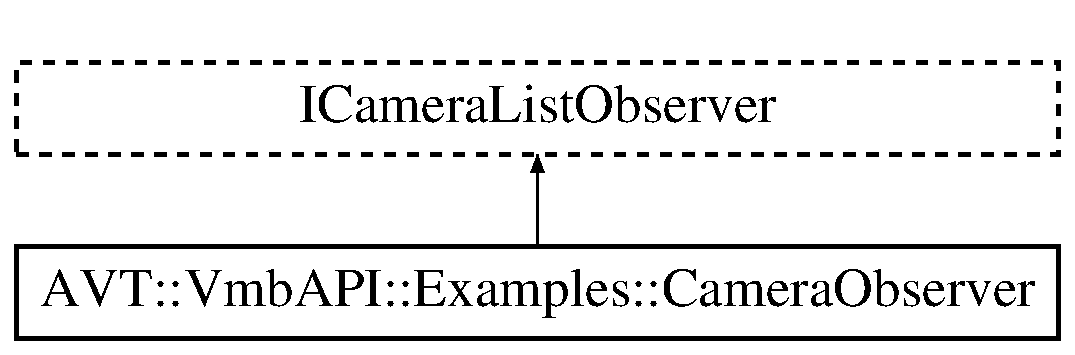
\includegraphics[height=2.000000cm]{class_a_v_t_1_1_vmb_a_p_i_1_1_examples_1_1_camera_observer}
\end{center}
\end{figure}
\subsection*{Public Member Functions}
\begin{DoxyCompactItemize}
\item 
\mbox{\Hypertarget{class_a_v_t_1_1_vmb_a_p_i_1_1_examples_1_1_camera_observer_af9ed70bae9b1477e177c5638a413247c}\label{class_a_v_t_1_1_vmb_a_p_i_1_1_examples_1_1_camera_observer_af9ed70bae9b1477e177c5638a413247c}} 
virtual void {\bfseries Camera\+List\+Changed} (Camera\+Ptr p\+Camera, Update\+Trigger\+Type reason)
\end{DoxyCompactItemize}


The documentation for this class was generated from the following files\+:\begin{DoxyCompactItemize}
\item 
Camera\+Observer.\+h\item 
Camera\+Observer.\+cpp\end{DoxyCompactItemize}

\hypertarget{class_c_asynchronous_grab_app}{}\section{C\+Asynchronous\+Grab\+App Class Reference}
\label{class_c_asynchronous_grab_app}\index{C\+Asynchronous\+Grab\+App@{C\+Asynchronous\+Grab\+App}}
Inheritance diagram for C\+Asynchronous\+Grab\+App\+:\begin{figure}[H]
\begin{center}
\leavevmode
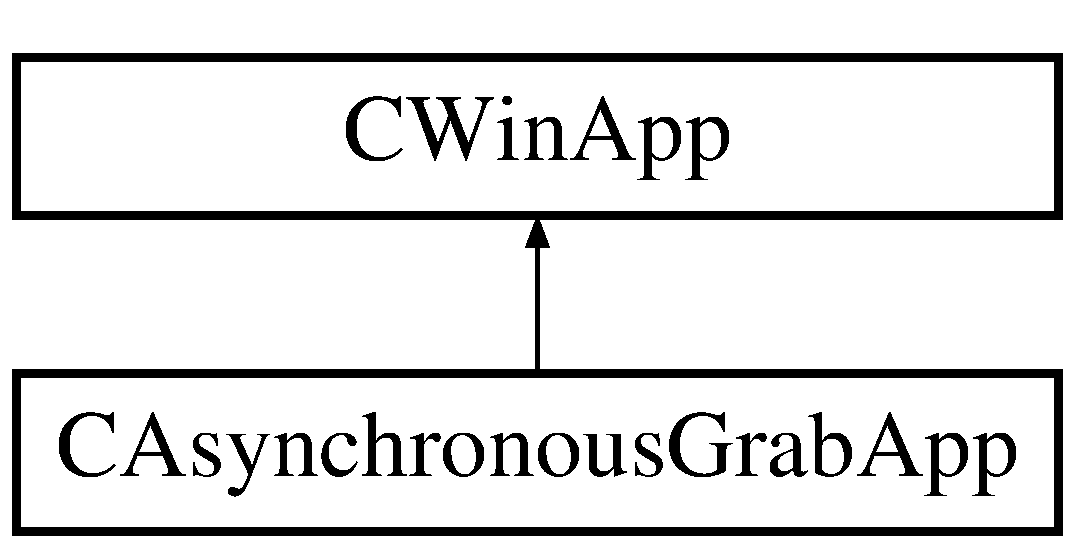
\includegraphics[height=2.000000cm]{class_c_asynchronous_grab_app}
\end{center}
\end{figure}
\subsection*{Public Member Functions}
\begin{DoxyCompactItemize}
\item 
\mbox{\Hypertarget{class_c_asynchronous_grab_app_a740832a02b08e1b68394718e5367b4b4}\label{class_c_asynchronous_grab_app_a740832a02b08e1b68394718e5367b4b4}} 
virtual B\+O\+OL {\bfseries Init\+Instance} ()
\end{DoxyCompactItemize}


The documentation for this class was generated from the following files\+:\begin{DoxyCompactItemize}
\item 
Asynchronous\+Grab.\+h\item 
Asynchronous\+Grab.\+cpp\end{DoxyCompactItemize}

\hypertarget{class_c_asynchronous_grab_dlg}{}\section{C\+Asynchronous\+Grab\+Dlg Class Reference}
\label{class_c_asynchronous_grab_dlg}\index{C\+Asynchronous\+Grab\+Dlg@{C\+Asynchronous\+Grab\+Dlg}}
Inheritance diagram for C\+Asynchronous\+Grab\+Dlg\+:\begin{figure}[H]
\begin{center}
\leavevmode
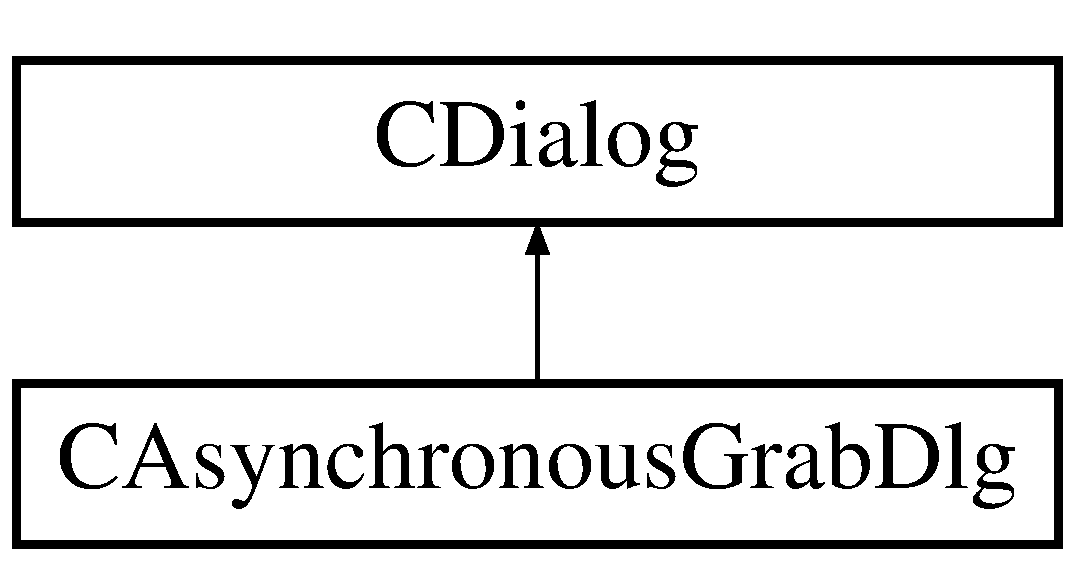
\includegraphics[height=2.000000cm]{class_c_asynchronous_grab_dlg}
\end{center}
\end{figure}
\subsection*{Public Types}
\begin{DoxyCompactItemize}
\item 
\mbox{\Hypertarget{class_c_asynchronous_grab_dlg_aa71938de5350ae71062a26f6f3506dca}\label{class_c_asynchronous_grab_dlg_aa71938de5350ae71062a26f6f3506dca}} 
enum \{ {\bfseries I\+DD} = I\+D\+D\+\_\+\+A\+S\+Y\+N\+C\+H\+R\+O\+N\+O\+U\+S\+G\+R\+A\+B\+\_\+\+D\+I\+A\+L\+OG
 \}
\end{DoxyCompactItemize}
\subsection*{Public Member Functions}
\begin{DoxyCompactItemize}
\item 
\mbox{\Hypertarget{class_c_asynchronous_grab_dlg_a2a8491d7e5e8dc44c359be44e8237c87}\label{class_c_asynchronous_grab_dlg_a2a8491d7e5e8dc44c359be44e8237c87}} 
{\bfseries C\+Asynchronous\+Grab\+Dlg} (C\+Wnd $\ast$p\+Parent=N\+U\+LL)
\end{DoxyCompactItemize}
\subsection*{Protected Member Functions}
\begin{DoxyCompactItemize}
\item 
\mbox{\Hypertarget{class_c_asynchronous_grab_dlg_af261b91107b56f5270f84f75287b701c}\label{class_c_asynchronous_grab_dlg_af261b91107b56f5270f84f75287b701c}} 
virtual void {\bfseries Do\+Data\+Exchange} (C\+Data\+Exchange $\ast$p\+DX)
\item 
\mbox{\Hypertarget{class_c_asynchronous_grab_dlg_abfdeb6b9745c723693bac476f2bb08c5}\label{class_c_asynchronous_grab_dlg_abfdeb6b9745c723693bac476f2bb08c5}} 
virtual B\+O\+OL {\bfseries On\+Init\+Dialog} ()
\item 
\mbox{\Hypertarget{class_c_asynchronous_grab_dlg_a27d395d8013249a9474b8cf764860275}\label{class_c_asynchronous_grab_dlg_a27d395d8013249a9474b8cf764860275}} 
afx\+\_\+msg void {\bfseries On\+Sys\+Command} (U\+I\+NT n\+ID, L\+P\+A\+R\+AM l\+Param)
\item 
\mbox{\Hypertarget{class_c_asynchronous_grab_dlg_ab2ae7237273e24f043805b73e0f2308c}\label{class_c_asynchronous_grab_dlg_ab2ae7237273e24f043805b73e0f2308c}} 
afx\+\_\+msg void {\bfseries On\+Paint} ()
\item 
\mbox{\Hypertarget{class_c_asynchronous_grab_dlg_a52181401d28bf6d2a5bb37f9122b82d3}\label{class_c_asynchronous_grab_dlg_a52181401d28bf6d2a5bb37f9122b82d3}} 
afx\+\_\+msg H\+C\+U\+R\+S\+OR {\bfseries On\+Query\+Drag\+Icon} ()
\item 
\mbox{\Hypertarget{class_c_asynchronous_grab_dlg_a0fe44529e4db12f1d59842d0ea107795}\label{class_c_asynchronous_grab_dlg_a0fe44529e4db12f1d59842d0ea107795}} 
afx\+\_\+msg void {\bfseries On\+Bn\+Clicked\+Button\+Startstop} ()
\item 
\mbox{\Hypertarget{class_c_asynchronous_grab_dlg_a93f307a8a9b94a2b214c3da1c3d3abf2}\label{class_c_asynchronous_grab_dlg_a93f307a8a9b94a2b214c3da1c3d3abf2}} 
afx\+\_\+msg L\+R\+E\+S\+U\+LT {\bfseries On\+Frame\+Ready} (W\+P\+A\+R\+AM status, L\+P\+A\+R\+AM l\+Param)
\item 
\mbox{\Hypertarget{class_c_asynchronous_grab_dlg_a939b1c7c3ad35fd78ff395749dbc9b5e}\label{class_c_asynchronous_grab_dlg_a939b1c7c3ad35fd78ff395749dbc9b5e}} 
afx\+\_\+msg L\+R\+E\+S\+U\+LT {\bfseries On\+Camera\+List\+Changed} (W\+P\+A\+R\+AM reason, L\+P\+A\+R\+AM l\+Param)
\end{DoxyCompactItemize}
\subsection*{Protected Attributes}
\begin{DoxyCompactItemize}
\item 
\mbox{\Hypertarget{class_c_asynchronous_grab_dlg_a26871f858f6a7157b6b2ccb765e37620}\label{class_c_asynchronous_grab_dlg_a26871f858f6a7157b6b2ccb765e37620}} 
H\+I\+C\+ON {\bfseries m\+\_\+h\+Icon}
\end{DoxyCompactItemize}


The documentation for this class was generated from the following files\+:\begin{DoxyCompactItemize}
\item 
Asynchronous\+Grab\+Dlg.\+h\item 
Asynchronous\+Grab\+Dlg.\+cpp\end{DoxyCompactItemize}

\hypertarget{class_a_v_t_1_1_vmb_a_p_i_1_1_examples_1_1_frame_observer}{}\section{A\+VT\+:\+:Vmb\+A\+PI\+:\+:Examples\+:\+:Frame\+Observer Class Reference}
\label{class_a_v_t_1_1_vmb_a_p_i_1_1_examples_1_1_frame_observer}\index{A\+V\+T\+::\+Vmb\+A\+P\+I\+::\+Examples\+::\+Frame\+Observer@{A\+V\+T\+::\+Vmb\+A\+P\+I\+::\+Examples\+::\+Frame\+Observer}}
Inheritance diagram for A\+VT\+:\+:Vmb\+A\+PI\+:\+:Examples\+:\+:Frame\+Observer\+:\begin{figure}[H]
\begin{center}
\leavevmode
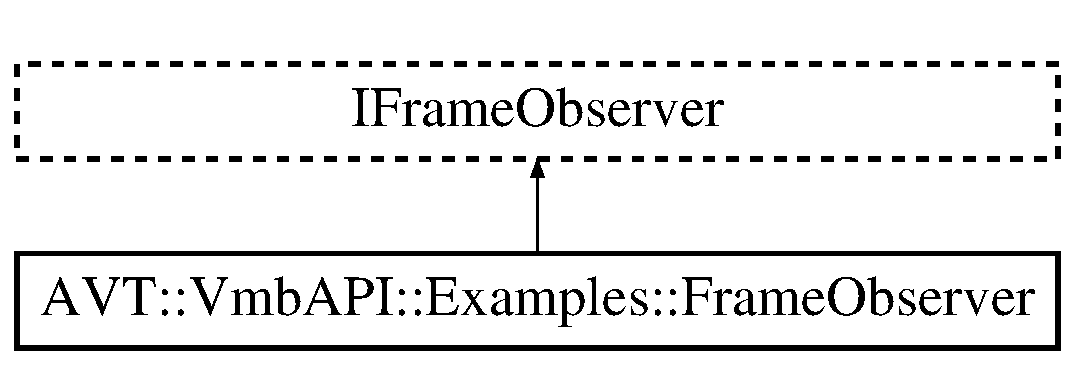
\includegraphics[height=2.000000cm]{class_a_v_t_1_1_vmb_a_p_i_1_1_examples_1_1_frame_observer}
\end{center}
\end{figure}
\subsection*{Public Member Functions}
\begin{DoxyCompactItemize}
\item 
\mbox{\Hypertarget{class_a_v_t_1_1_vmb_a_p_i_1_1_examples_1_1_frame_observer_a28b23d2b16c95929ee4463bd0ba8f867}\label{class_a_v_t_1_1_vmb_a_p_i_1_1_examples_1_1_frame_observer_a28b23d2b16c95929ee4463bd0ba8f867}} 
{\bfseries Frame\+Observer} (Camera\+Ptr p\+Camera)
\item 
\mbox{\Hypertarget{class_a_v_t_1_1_vmb_a_p_i_1_1_examples_1_1_frame_observer_a09bfd28da454e248621496663e8c1e7d}\label{class_a_v_t_1_1_vmb_a_p_i_1_1_examples_1_1_frame_observer_a09bfd28da454e248621496663e8c1e7d}} 
virtual void {\bfseries Frame\+Received} (const Frame\+Ptr p\+Frame)
\item 
\mbox{\Hypertarget{class_a_v_t_1_1_vmb_a_p_i_1_1_examples_1_1_frame_observer_ae932f5adb14ae6cc88bbc335759b37eb}\label{class_a_v_t_1_1_vmb_a_p_i_1_1_examples_1_1_frame_observer_ae932f5adb14ae6cc88bbc335759b37eb}} 
Frame\+Ptr {\bfseries Get\+Frame} ()
\item 
\mbox{\Hypertarget{class_a_v_t_1_1_vmb_a_p_i_1_1_examples_1_1_frame_observer_a3b6e1c1643170b09de173fe7506d409d}\label{class_a_v_t_1_1_vmb_a_p_i_1_1_examples_1_1_frame_observer_a3b6e1c1643170b09de173fe7506d409d}} 
void {\bfseries Clear\+Frame\+Queue} ()
\end{DoxyCompactItemize}


The documentation for this class was generated from the following files\+:\begin{DoxyCompactItemize}
\item 
Frame\+Observer.\+h\item 
Frame\+Observer.\+cpp\end{DoxyCompactItemize}

%--- End generated contents ---

% Index
\backmatter
\newpage
\phantomsection
\clearemptydoublepage
\addcontentsline{toc}{chapter}{Index}
\printindex

\end{document}
